\section{Reference Trajectory}
\label{sec:reftraj}
%
The reference trajectory is dissected into eight parts, as seen in
Figure~\ref{fig:motion_plan}. We describe each frame and the transitions between
them in the following subsections. 
%
\begin{figure*}[tb]
  \centering
  % \includegraphics[width=0.45\textwidth]{./figures/.eps}
  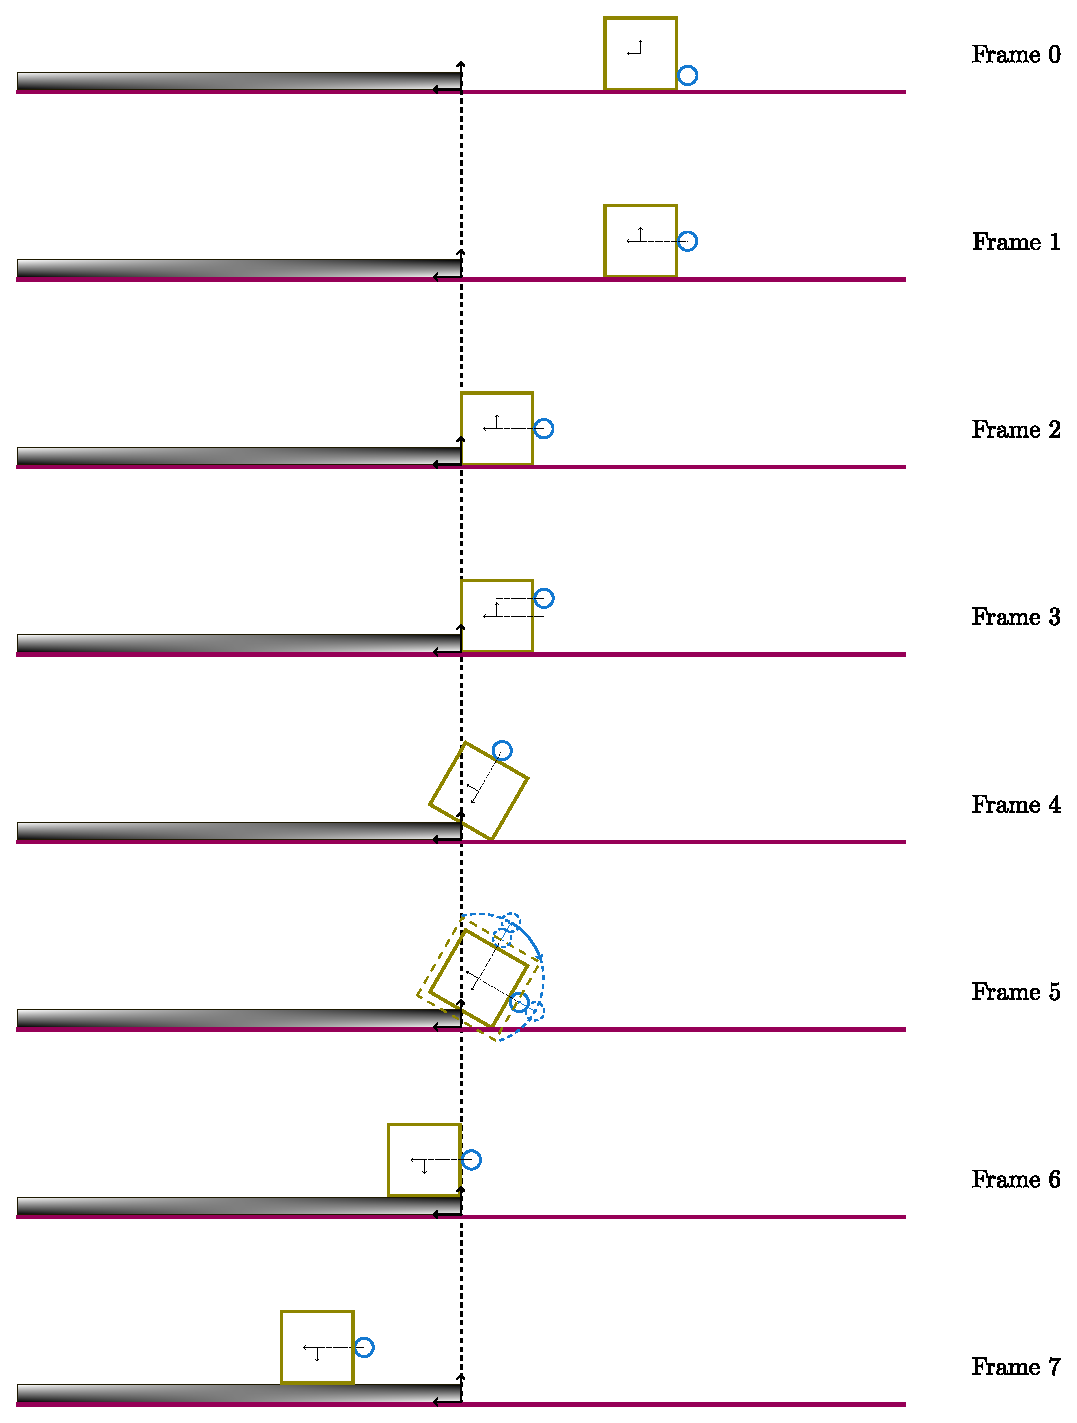
\includegraphics[width=0.731\textheight]{./figures/motion_plan_v1.eps}
  \caption{Motion plan} 
  \label{fig:motion_plan}
\end{figure*}
%

\subsection{Frame 0 to Frame 1}
\label{sec:frame0to1}
%
Frame $0$ is the initial condition. This condition is generated by sampling 
as follows:
%
\begin{itemize}
  \item Sample the box's $x$-position: 
  $x_b \sim \mc{U}\left(-\ell, -\nicefrac{1}{2}\right)$.
  \item The box's $z$-position is fixed at $z_b = \ell$.
  \item The box's rotation is fixed at $\theta_b = 0$.
  \item The manipulator's $x$-position is fixed at $x_m = x_b - \ell - r$.
  \item Sample the manipulator's $z$-position:
  $z_m ~\sim \mc{U}\left(\nicefrac{\ell}{2}, \nicefrac{3\ell}{2}\right)$.
\end{itemize}
%
We transition from frame $0$ to frame $1$ by moving the manipulator to the
geometric center of the box in the $z$-direction, i.e., the plan is executed 
by~\eqref{eq:frame0to1}
\begin{equation}
  z_m(t; t_0) = \lininterp\left(z_m(t_0), \ell, t; \, t_0\right).
  \label{eq:frame0to1}
\end{equation}
%
Other coordinates are fixed during this transition. 


\subsection{Frame 1 to Frame 2}
\label{sec:frame1to2}
%
The transition from frame $1$ to frame $2$ involves moving the box snug against
the step. This plan is executed by the following motion~\eqref{eq:frame1to2}
%
\begin{align}
\begin{split}
  x_b(t; t_1) &= \lininterp\left(x_b(t_1), -\ell, t; \, t_1\right), \\
  x_m(t; t_1) &= \lininterp\left(x_m(t_1), -2\ell-r, t; \, t_1\right). \\
\end{split}
  \label{eq:frame1to2}
\end{align}
%
Other coordinates are fixed during this transition. 


\subsection{Frame 2 to Frame 3}
\label{sec:frame2to3}
%
The transition from frame $2$ to frame $3$ involves moving the manipulator above
the center of mass of the box, so that it can produce torque on the box by
pushing it. This plan is executed by the following motion~\eqref{eq:frame2to3}
%
\begin{equation}
  z_m(t; t_2) = \lininterp\left(z_m(t_2), \nicefrac{3\ell}{2}, t; \, t_2\right).
  \label{eq:frame2to3}
\end{equation}
%
Other coordinates are fixed during this transition.


\subsection{Frame 3 to Frame 4}
\label{sec:frame3to4}
%
During this transition, the box will rotate by approximately $60^\circ$, while 
the manipulator moves back to the level of the center of mass of the box so that
at the end of the transition, it cannot produce torque on the box by simply
pushing on it in the normal direction.

This is a more complicated motion when represented in the inertial frame. We
first compute the location of the center of the box as a function of its 
rotation, assuming that the bottom left corner of the box remains on the floor 
and a point of the box remains in contact with the step. Hence, the box 
position, as a function of its rotation $\theta_b$, is given by
%
\[ \bm{p}_b = \bm{p}_a  + \ell\bm{R}\bmat{-1 \\ 1} = \bmat{
  -2h \tan{\theta_b} + \ell(s_b - c_b) \\ \ell(c_b + s_b)
}, \]
%
where $\bm{p}_a$ is the position of the bottom left corner of the box, given by
$\bm{p}_a = \bmat{-2h \tan{\theta_b} & 0}^\top$. The rotation matrix $\bm{R}$ is
as given in equation~\eqref{eq:pose_box}. Given a trajectory for $\theta_b$,
this equation gives the corresponding trajectory for the box location, $p_b$.

The corresponding trajectory for the manipulator can be deduced by our previous 
work in Section~\ref{sec:sampling}. It is given by 
%
\[
  \bm{p}_m = \bm{p}_b + \bm{R}\bmat{
    -\ell - r \\ \ell \tan{\theta_m},
  } = 
  \bmat{
    x_b - (\ell + r) c_b + \ell \tan{(\theta_m)} s_b \\
    z_b + (\ell + r) s_b + \ell \tan{(\theta_m)} c_b
  }.
\]
%
where $\theta_m$ is the angle between the manipulator's $x$-axis and the 
position vector from the box's origin to the manipulator's origin. Due to the 
construction in frame $3$, $\theta_m$ starts at $\pi + \arctan{\nicefrac{1}{2}}$
and ends at $\theta_m = \pi$.

Hence, the transition from frame $3$ to frame $4$ is given by the following
motion~\eqref{eq:frame3to4}
%
\begin{equation}
  \begin{split}
    \theta_b(t; t_3) &= \lininterp\left(0, \nicefrac{\pi}{3}, t; \, t_3\right), \\
    \theta_m(t; t_3) &= \lininterp\left(\pi + \arctan{\nicefrac{1}{2}}, \pi, t; \, t_3\right).
  \end{split}
  \label{eq:frame3to4}
\end{equation}
%
The translation vectors of the box and the manipulator are given by the 
two previous equations above.


\subsection{Frame 4 to Frame 5}
\label{sec:frame4to5}
%
This transition assumes that the box is stationary and is concerned with moving 
the manipulator in a convenient location to keep pushing the box up the step. 
We will execute this step by moving the manipulator along a circumscribed
circle $\mc{C}$, with center at the center of the box and radius equal to
$\sqrt{2}(\ell + r)$.  This will be executed in three phases: (i) radially move
the manipulator to $\mc{C}$, (ii) rotate the manipulator around the center of
the box by $\nicefrac{\pi}{2}$, and (iii) radially move the manipulator to the
``bottom'' face of the box.

\subsubsection{Phase 1: Move to $\mc{C}$}
%
Note that at $t = t_4$, we have 
\[ \bm{p}_m(t_4) = \bm{p}_b(t_4) - (\ell+r)\bm{R}\bmat{1 \\ 0}, \] hence
the desired motion is achieved by the following linear interpolation
\[
\bm{p}_m(t; t_4) = \lininterp\,\left(\bm{p}_m(t_4), \bm{p}_b - \sqrt{2}(\ell +
r)\bm{R}\bmat{1 \\ 0}, t; t_4\right).  
\]

\subsubsection{Phase 2: Rotate around the center of the box}
%
This is achieved by the following linear interpolation
\[
\theta(t; t_4^{\prime}) = \lininterp\left(\theta_b+\pi,
\theta_b+\nicefrac{\pi}{2}, t; t_4^\prime \right),
\]
%
and
\[
\bm{p}_m(t; t_4^{\prime}) = \bm{p}_b + \sqrt{2}(\ell +
r)\bm{R}_{y,\theta}\bmat{1 \\ 0}.
\]

\subsubsection{Phase 3: Move to the bottom face of the box}
%
Note that at $t = t_4^{\prime\prime}$, we have 
\[ \bm{p}_m(t_4^{\prime\prime}) = \bm{p}_b(t_4^{\prime\prime}) -
\sqrt{2}(\ell+r)\bm{R}\bmat{0 \\ 1}, \] hence the desired motion is
achieved by the following linear interpolation
\[ 
\bm{p}_m(t; t_4^{\prime\prime}) =
\lininterp\,\left(\bm{p}_m(t_4^{\prime\prime}), \bm{p}_b - (\ell+r)\bm{R}\bmat{0
\\ 1}, t; t_4^{\prime\prime}\right).
\]
%
Other coordinates are fixed during this transition. 

\subsection{Frame 5 to Frame 6}
\label{sec:frame5to6}
%
The transition from frame $5$ to frame $6$ involves moving the box on top of the
step by pushing it without exerting torque on it. This plan can be executed, to 
a good approximation, by the following motion plan.
%
\begin{align}
\begin{split}
  \theta_b(t; t_5) &= \lininterp\left(\nicefrac{\pi}{3}, \nicefrac{\pi}{2}, t;
  t_5\right), \\
  \bm{p}_b(t; t_5) &= \lininterp\left(\bm{p}_b(t_5), \bmat{\ell & \ell +
  2h}^\top, t; t_5\right), \\
  \bm{p}_m(t; t_5) &= \lininterp\left(\bm{p}_m(t_5), \bmat{-r & \ell +
  2h}^\top, t; t_5\right).
\end{split}
  \label{eq:frame5to6}
\end{align}
%

\subsection{Frame 6 to Frame 7}
\label{sec:frame6to7}
%
Finally, the transition from frame $6$ to frame $7$ simply moves the box's $x$-
position from $\ell$ to $\nicefrac{1}{4}$. This is achieved by the linear
interpolation
%
\begin{align}
\begin{split}
  x_b(t; t_6) &= \lininterp\left(\ell, \nicefrac{1}{4}, t; t_6\right), \\
  x_m(t; t_6) &= \lininterp\left(-r, \nicefrac{1}{4}-\ell-r, t; t_6\right).
\end{split}
  \label{eq:frame6to7}
\end{align}
%
Other coordinates are fixed during this transition.